
\section{Model calculations and proofs}

\subsection{Value functions of the Citizens and the Elites}\label{section:bellman_app}

Both the Elites and the Citizens have \citeauthor{Epstein1989} utility over output. For the Citizens, in autocracy, their only decision is over whether to revolt; in democracy their only decision is the tax rate to implement. To understand the former, we need to understand the solution to the Citizens' value function. We can solve this in three cases: (1) by solving for their value function in the revolution, (2) by solving for their value function in democracy, and (3) by solving for their value function in autocracy as a function of the cost of revolution $\mu$. For the Elites, they must decide the tax rate to set in autocracy, and make no decisions of consequence for the political environment in democracy. In all periods, they must choose their portfolio in financial markets.

\paragraph{Value functions in the revolution}
If the Citizens decide to revolt, their value function can be written as
\begin{equation*}
V^{p}(R,\mu_{t})^{1-1/\psi}=(1-\beta)(Y_{t}^{R})^{1-1/\psi}+\beta\left(\mathbb{E}_{t}\left[V^{p}(R,\mu_{t})^{1-\gamma}\right]\right)^{\frac{1-1/\psi}{1-\gamma}}
\end{equation*}
where $Y^R \equiv \big(\frac{1-\mu}{1-\delta}\big) Y$ and the expectation is taken over the next period value of $Y$. Because $Y$ is independent and identically distributed and the value function is homogeneous, we can scale the value function by $Y$, which yields $v^{p}(R,\mu_t)Y_t \equiv V^{p}(R,\mu_t)$. The scaled value function is then equal to:
\begin{equation*}
v^{p}(R,\mu_{t})^{1-1/\psi}=(1-\beta)\bigg(\frac{1-\mu_t}{1-\delta}\bigg)^{1-1/\psi}+\beta^{\star}\left(v^{p}(R,\mu_{t})^{1-\gamma}\right)^{\frac{1-1/\psi}{1-\gamma}}
\end{equation*}
where $\beta^{\star}=\beta e^{(1-1/\psi)\bar{y}+\frac{1}{2}(1-\gamma)(1-1/\psi)\sigma_{y}^{2}}$. Solving for the value function yields the solution,
\begin{equation*}
v^{p}(R,\mu_{t})=\bigg(\frac{1-\beta}{1-\beta^{\star}}\bigg)^{\frac{1}{1-1/\psi}}\bigg(\frac{1-\mu_t}{1-\delta}\bigg).
\end{equation*}
The Elites conversely are assumed to have a large negative payoff in the revolution state $v^r(R)$ such that they would always rather concede democracy.

\paragraph{Value functions in democracy}
The value function of the Citizens in democracy can be solved for using an identical logic to the solution in the revolution. Since the economy remains a democracy forever after a successful democratization, the value function can be written as
\begin{equation*}
v^{p}(D)^{1-1/\psi}=(1-\beta)\hat{y}^{p} (\tau^{p*},\theta^{D},\nu^D)^{1-1/\psi}+\beta^{\star}\left(v^{p}(D)^{1-\gamma}\right)^{\frac{1-1/\psi}{1-\gamma}}.
\end{equation*}
Solving yields
\begin{equation*}
v^{p}(D)=\bigg(\frac{1-\beta}{1-\beta^{\star}}\bigg)^{\frac{1}{1-1/\psi}}\hat{y}^{p} (\tau^{p*},\theta^{D},\nu^D).
\end{equation*}
%where the term multiplying $\beta^{\star}$ takes into account the differences in growth in the two political regimes.

In equilibrium, the value function of the Elites in democracy can be solved for in the same way and is given by
\begin{equation*}
v^{r}(D)=\bigg(\frac{1-\beta}{1-\beta^{\star}}\bigg)^{\frac{1}{1-1/\psi}}\hat{y}^{r} (\tau^{p*},\theta^{D},\nu^D).
\end{equation*}


\paragraph{Value to the Citizens in autocracy}
In autocracy, there will be a solution to the value function for each value $\mu$ takes.  This means we can write the value function of the Citizens in autocracy as
\begin{equation}
	v^{p}(A,\mu_{t})^{1-1/\psi}=(1-\beta)\hat{y}_{t}^{p}(\tau_{t},\theta^{A},\nu^A)^{1-1/\psi}+\beta^{\star}\left(\mathbb{E}_{t}\left[v^p(\mu_{t+1})^{1-\gamma}\right]\right)^{\frac{1-1/\psi}{1-\gamma}}
\end{equation}
where the continuation value is given by
\begin{equation*}
		v^p(\mu_{t+1})=\begin{cases}
v^{p}(D)^{1-\gamma} & \text{if } \phi_{t+1} = 1 \\
v^{p}(A,\mu_{t+1})^{1-\gamma} & \text{if }\phi_{t+1} = 0 \\
v^{p}(R,\mu_{t+1})^{1-\gamma} & \text{if }\rho_{t+1} = 1
\end{cases}.
\end{equation*}

\paragraph{Value function of the Elites in autocracy}

The Elites have \citeauthor{Epstein1989} utility and trade in the consumption claim and a zero-net supply riskfree bond. The recursive formulation of their utility in autocracy can be written similar to the Citizens' utility and is given by
\begin{equation}
	v^{r}(A,\mu_{t})^{1-1/\psi}=(1-\beta)(\hat{y}^{r} (\tau_t,\theta^{A},\nu^A))^{1-1/\psi}+\beta^{\star}\left(\mathbb{E}_{t}\left[v^r(\mu_{t+1})^{1-\gamma}\right]\right)^{\frac{1-1/\psi}{1-\gamma}}
\end{equation}
where
\begin{equation*}
v^r(\mu_{t+1})=\begin{cases}
v^{r}(D)^{1-\gamma} & \text{if } \phi_{t+1} = 1 \\
v^{r}(A,\mu_{t+1}) & \text{if }\phi_{t+1} = 0 \\
v^r(R) & \text{if }\rho_{t+1} = 1
\end{cases}
\end{equation*}
with $v^r(R)$ representing the utility of the Elites in the revolution which does not depend on $\mu$. The budget constraint is the standard relation
\begin{equation}
W_{t+1} = (W_t-C_t^r)R_{W,t+1}
\label{eq:budgetconstraint_ez}
\end{equation}
and market clearing requires that Elite income equals Elite consumption in the aggregate and that the aggregate Elite portfolio place a weight of 1 on the consumption claim (following from the riskfree asset being in zero-net supply). This is because there is no trading between the Elites and the Citizens in autocracy. The pricing kernel revolves around the growth rate of the consumption of the Elites. This can be decomposed as
\begin{equation}
\log \bigg(\frac{C_{t+1}^r}{C_{t}^r} \bigg) \equiv \log \bigg(\frac{Y_{t+1}}{Y_{t}}\bigg)- \log\left(\frac{c_{t+1}^{r}}{c_{t}^{r}}\right)
\end{equation}
where $c^r$ is Elite consumption relative to aggregate income. The growth rate of this is given by
\begin{equation}
 \chi_{t+1} \equiv \log \frac{c_{t+1}^{r}}{c_{t}^{r}} = \begin{cases} 
\log Z & \textrm{if }\phi_{t}=1;\phi_{t-1}=0 \\
0 & \textrm{otherwise}
\end{cases} 
\end{equation}
where $Z<1$ represents the penalty the Elites face to their consumption upon a successful transition to democracy, given by
\begin{equation}
	Z= \frac{\hat{y}^{r} (\tau^{p*},\theta^{D},\nu^D)}{\hat{y}^{r} (\tau_t,\theta^{A},\nu^A)}.
\end{equation}

\subsection{Solution to more general cases of the model}\label{section:generalCase}

In the main text, the model is calibrated such that upon reaching the third state, society transitions to democracy. In general though, for higher values of $\mu$ in the third state, the outcomes will be different. This section solves for the cutoff values of $\mu$ that achieve the different equilibrium outcomes in the third state, in particular, the three thresholds, $\underbar{\ensuremath{\mu}}$, $\mu^{*}$, and $\mu^{D}$. In this example, for simplicity I take the case where $\mu^1 = \mu^2 = 1$ and $\mu^3 = \mu$, and I will characterize the solution for the threshold points in the third state. Further, also assume $\omega=1$ and $\nu=\delta$ to simplify the math. The transition matrix is given by
\begin{equation*}
\mathbf{P}=\begin{pmatrix}
p_{11} & p_{12} & p_{13} \\
p_{21} & p_{22} & p_{23} \\
p_{31} & p_{32} & p_{33} 
\end{pmatrix}
\end{equation*}
where all of the rows must sum to 1. The optimized value function (scaled by $Y$) of the citizens can be expressed compactly as
\begin{equation*}
\mathbf{V}^p = \mathbf{Y} + \beta^\star \mathbf{P}\mathbf{V}^p
\end{equation*}
and implies the solution
\begin{equation}
\mathbf{V}^p =(\mathbf{I}-\beta^\star \mathbf{P})^{-1} \mathbf{Y}
\end{equation}
where $\mathbf{I}$ is the identity matrix. The solutions in this case are pinned down by the cashflows in the final state and the transition probabilities.

To obtain the first threshold, $\underbar{\ensuremath{\mu}}$, notice that the present value of consumption when the Citizens receive no transfers in any period is
\begin{equation}
V^{p}(A,\mu_{t}; \tau_t = 0 \; \forall t) =\frac{1-\theta^A}{(1-\delta)(1-\beta^{\star})}.\label{eq:statusquo} \\
\end{equation}
Equating Equation (\ref{eq:revolution}) with Equation (\ref{eq:statusquo}) shows that 
\begin{equation}
\underbar{\ensuremath{\mu}} = \theta^A.\label{eq:muunderbar}
\end{equation} 
The second threshold, $\mu^*$, is given by
\begin{equation}
\mu^* =\theta^A-\frac{\varpi(\theta^A-\delta)^2}{2(1-\delta)},\label{eq:mustar}
\end{equation}
where
%\label{eq:consterm}
\begin{align*}
\varpi & =  \mathbf{e}_3^\prime(\mathbf{I}-\beta^\star \mathbf{P})^{-1} \mathbf{e}_3(1-\beta^\star)
\end{align*}
where $\mathbf{e}_3$ is a column vector with a 1 in the third position and zeros elsewhere, $\mathbf{I}$ is a $3\times 3$ identity matrix.  In addition, when $\mu$ is in the range $\mu \in [\mu^{*},\underbar{\ensuremath{\mu}})$, the minimum tax the Elites can offer to avoid revolution is given by
\begin{equation}
\hat{\tau}(\mu) =\frac{\theta^A-\delta}{1-\delta} - \frac{\sqrt{\left(\theta^A-\delta\right)^2 - 2\left(\frac{\theta^A-\mu}{\varpi}\right)(1-\delta)}}{1-\delta}.\label{eq:mintax}
\end{equation}
The final threshold, $\mu^{D}$ is described above in Equation (\ref{eq:mudoublestar}).

\begin{prop}
If the transition matrix for $\mu$ follows Equation (\ref{eq:transmat}) and $\mu^{1}=\mu^{2}=1$ and $\mu^{3}=\mu$, and the regularity conditions $\beta^{\star}<1$ and $\theta>\delta$ hold, then: 
\begin{itemize}
	\item For $\mu \in [\underbar{\ensuremath{\mu}},1]$, the economy is an autocracy and taxes are set to 0 in all periods;
	\item For $\mu \in [\mu^{*},\underbar{\ensuremath{\mu}})$, the economy is an autocracy in all periods and taxes are set to 0 in the autocracy state and the democratization state, and to $\hat{\tau}(\mu)$, as specified in Equation (\ref{eq:mintax}), in the third state;
	\item For $\mu \in [\mu^{D},\mu^{*})$, the economy is an autocracy and taxes are set to 0 in the autocracy state and the democratization state, and the economy becomes a democracy in the third state and taxes are set to $\tau^{p*}$. Once the third state is reached, the economy remains a democracy forever;
	\item For $\mu \in [0,\mu^{D})$, the economy is an autocracy and taxes are set to 0 in the autocracy state and the democratization state, and the Citizens revolt in the third state;
\end{itemize}
is a Markov perfect equilibrium with the threshold points $\underbar{\ensuremath{\mu}}$, $\mu^{*}$, and $\mu^{D}$ described by Equations (\ref{eq:muunderbar}), (\ref{eq:mustar}), and (\ref{eq:mudoublestar}). The associated thresholds and the states they correspond to are shown in Figure~\ref{fig:mu_graph}.
\end{prop}

\begin{figure}[b!]
	\caption{\textbf{Equilibrium Outcome for Regions of $\mu$} }
	\renewcommand{\baselinestretch}{1}
	\label{fig:mu_graph}
	\footnotesize
    \begin{center}
    \addtolength{\leftskip} {-.65cm}
    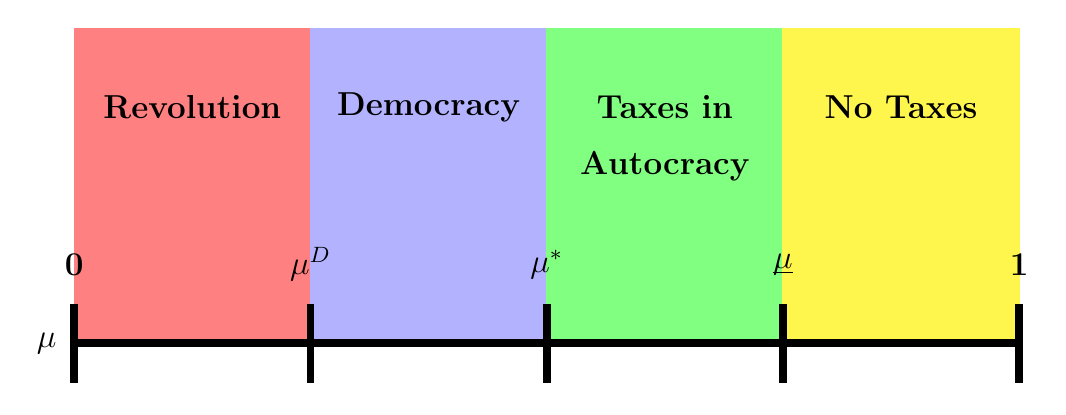
\begin{tikzpicture}	
		\draw[draw = red!50,fill=red!50] (-2,0) -- (1,0) -- (1,4) -- (-2,4) -- (-2,0);
		\draw[draw= blue!30,fill=blue!30] (1,0) -- (4,0) -- (4,4) -- (1,4) -- (1,0);
		\draw[draw=green!50, fill=green!50] (4,0) -- (7,0) -- (7,4) -- (4,4) -- (4,0);
		\draw[draw= yellow!70,fill = yellow!70] (7,0) -- (10,0) -- (10,4) -- (7,4) -- (7,0);
		\node[very thick,align=center,black] (r4) at (4,1)  {\large{$\mu^{*}$}};
		\draw[line width = 1mm] (4,.5) -- (4,-.5);
		\node[very thick,align=center,black] (r4) at (7,1)  {\large{$\mathbf{\underbar{\ensuremath{\mu}}}$}};
		\draw[line width = 1mm] (7,.5) -- (7,-.5);
		\node[very thick,align=center,black] (r4) at (1,1)  {\large{$\mu^{D}$}};
		\draw[line width = 1mm] (1,.5) -- (1,-.5);
		\node[very thick,align=center,black] (r4) at (5.5,3)  {\large{\bf Taxes in}};
		\node[very thick,align=center,black] (r4) at (5.5,2.25)  {\large{\bf Autocracy}};
		\node[very thick,align=center,black] (r4) at (8.5,3)  {\large{\bf No Taxes}};
		\node[very thick,align=center,black] (r4) at (2.5,3)  {\large{\bf Democracy}};
		\node[very thick,align=center,black] (r4) at (-0.5,3)  {\large{\bf Revolution}};
		\draw[line width = 1mm] (-2,0) -- (10,0);
		\draw[line width = 1mm] (-2,.5) -- (-2,-.5);
		\draw[line width = 1mm] (10,.5) -- (10,-.5);
		\node[very thick,align=center,black] (r4) at (-2.35,0) {\large{$\mu$}};
		\node[very thick,align=center,black] (r4) at (-2,1) {\large{\bf 0}};
		\node[very thick,align=center,black] (r4) at (10,1) {\large{\bf 1}};
	\end{tikzpicture}	
	\end{center}
\end{figure}


\subsection{Asset pricing algebra}\label{section:ap4state}

The solution for the pricing kernel revolves around the growth rate of the consumption of the Elites. This can be decomposed as
\begin{equation}
\frac{C_{t+1}^r}{C_{t}^r} \equiv \bigg(\frac{Y_{t+1}}{Y_{t}}\bigg)\left(\frac{c_{t+1}^{r}}{c_{t}^{r}}\right)
\end{equation}
where $c_{t+1}$ is consumption scaled by aggregate income. The growth rate of scaled consumption is given by
\begin{equation}
\frac{c_{t+1}^{r}}{c_{t}^{r}}\equiv \begin{cases} 
Z & \textrm{if }\phi_{t}=1;\phi_{t-1}=0 \\
1 & \textrm{otherwise}
\end{cases} 
\end{equation}
where $Z<1$ represents the penalty the Elites face to their consumption upon a successful transition to democracy. This can take on two values, given by
\begin{equation}
Z \equiv \begin{cases} 
 Z_H = \frac{\hat{y}^{r} (\tau^{pH*},\theta^{DH},\nu^{DH})}{\hat{y}^{r} (\tau_t,\theta^{A},\nu^A)}. & \textrm{with probability }q \\
 Z_L = \frac{\hat{y}^{r} (\tau^{pL*},\theta^{DL},\nu^{DL})}{\hat{y}^{r} (\tau_t,\theta^{A},\nu^A)}. & \textrm{with probability } 1-q \\
\end{cases} 
\end{equation}
Under Epstein-Zin utility, the stochastic discount factor of the Elites is
\[
M_{t+1}=\beta^{\alpha}\bigg(\frac{C_{t+1}^r}{C_{t}^r}\bigg)^{-\frac{\alpha}{\psi}}R_{W,t+1}^{(\alpha-1)}
\]
where $\alpha \equiv \frac{1-\gamma}{1-\frac{1}{\psi}}$. The return on wealth can be written as
\begin{equation}
R_{W,t+1} = \bigg(\frac{\kappa_{t+1}}{\kappa_t - 1}\bigg)\bigg(\frac{C_{t+1}^r}{C_{t}^r}\bigg)
\end{equation}
where $\kappa \equiv W/C$ is the cum-dividend wealth-consumption ratio. Conjecture that $\kappa$ is constant in each state of $\mu$. This means that the solution is given by the solution to the system of equations
\begin{equation}
\kappa(\mu^j)=1+\beta e^{(1-\frac{1}{\psi})\bar{y}+\frac{1}{2}(1-\gamma)(1-\frac{1}{\psi})\sigma_y^2} \bigg[\mathbf{e}_j^\prime \mathbf{P}\boldsymbol\kappa^{\alpha}\bigg]^{\frac{1}{\alpha}}
\end{equation}
in states 1 and 2, where
\begin{equation}
\boldsymbol{\kappa}^{\alpha}\equiv\begin{pmatrix}\kappa(\mu^{1})^{\alpha}\\
\kappa(\mu^{2})^{\alpha}\\
\kappa(\mu^{3})^{\alpha}(qZ_H^{1-\gamma} + (1-q)Z_L^{1-\gamma})
\end{pmatrix}.
\end{equation}
In state 3, the wealth-consumption ratio is
$$
\kappa(\mu^{3})=\frac{1}{1-\beta e^{(1-\frac{1}{\psi})\bar{y}+\frac{1}{2}(1-\gamma)(1-\frac{1}{\psi})\sigma_y^{2}}}.
$$
This system of equations can be solved numerically.

The riskfree rate, similar to the wealth-consumption ratio, varies only with the state of $\mu$ and is given by
\begin{align*}
R_{f}(\mu_t) = \E\bigg[\beta^{\alpha}\bigg(\frac{C^r_{t+1}}{C^r_{t}}\bigg)^{-\gamma}\bigg(\frac{\kappa(\mu_{t+1})}{\kappa(\mu_{t})-1}\bigg)^{\alpha-1}\bigg]^{-1}.
\end{align*}
This once again yields a system of 3 equations for the riskfree rate, which are characterized by
\begin{equation}
R_{f}(\mu^{j})= \beta^{-\alpha}e^{\gamma\bar{y} -\frac{1}{2}\gamma^2 \sigma_y^2}\left(\kappa(\mu^{j})-1\right)^{\alpha-1}\bigg[\mathbf{e}_j^\prime \mathbf{P}\boldsymbol\kappa^{\alpha-1}\bigg]^{-1}
\end{equation}
in states 1 and 2, where
\begin{equation}
\boldsymbol{\kappa}^{\alpha-1}\equiv\begin{pmatrix}\kappa(\mu^{1})^{\alpha-1}\\
\kappa(\mu^{2})^{\alpha-1}\\
\kappa(\mu^{3})^{\alpha-1}(qZ_H^{-\gamma} + (1-q)Z_L^{-\gamma})
\end{pmatrix}.
\end{equation}
This riskfree rate in the 3rd state is given by
\begin{equation*}
R_{f}(\mu^3)= \beta^{-1}e^{\frac{1}{\psi}\bar{y} - \frac{1}{2}(\gamma-\frac{1}{\psi}(1-\gamma))\sigma_y^2}.
\end{equation*}

Recall that the dividend claim follows:
\begin{equation*}
\frac{D_{t+1}}{D_{t}} \equiv \bigg(\frac{Y_{t+1}}{Y_{t}}\bigg)^{\Upsilon}\chi^D_{t+1}.
\end{equation*}
This implies that the price-dividend ratio can be expressed as
\begin{equation}
1=\mathbb{E}_t\bigg[\beta^{\alpha}\bigg(\frac{C_{t+1}}{C_{t}}\bigg)^{\Upsilon-\gamma}\bigg(\frac{\kappa_{t+1}}{\kappa_t - 1}\bigg)^{(\alpha-1)} \chi^{-\gamma}_{t+1}\chi^D_{t+1} \bigg(\frac{pd_{t+1}+1}{pd_{t}}\bigg)\bigg]
\end{equation}
where $pd$ is the ex-dividend price-dividend ratio. In democracy, the price-dividend ratio is given by
\begin{equation}
pd(D) = \beta e^{(\Upsilon-\frac{1}{\psi})\bar{y}+\frac{1}{2}((\Upsilon-\gamma)^2 + (1-\gamma)(\gamma-\frac{1}{\psi}))\sigma_y^{2}} \bigg(pd_{t+1}+1\bigg)
\end{equation}
which implies that 
\begin{equation}
pd(D) = \frac{\beta e^{(\Upsilon-\frac{1}{\psi})\bar{y}+\frac{1}{2}((\Upsilon-\gamma)^2 + (1-\gamma)(\gamma-\frac{1}{\psi}))\sigma_y^{2}}}{1-\beta e^{(\Upsilon-\frac{1}{\psi})\bar{y}+\frac{1}{2}((\Upsilon-\gamma)^2 + (1-\gamma)(\gamma-\frac{1}{\psi}))\sigma_y^{2}}}.
\end{equation}

\subsection{Gradual redistribution}\label{section:gradual_redist}

In actual democratizations redistribution happens gradually. However, in the model in the main text, redistribution happens all at once upon the conclusion of a successful transition to democracy. This appendix section reformulates the model to allow for more gradual redistribution. Here, we have Elite consumption following the same as in Equation (\ref{eq:elite_consumption}) by $\chi$ is now equal to
\begin{equation}
\chi_{t+1} \equiv \begin{cases} 
e^{- \bar{y}^r} & \textrm{if }\phi_{t}=1 \\
1 & \textrm{otherwise}
\end{cases}.
\end{equation}
Here, $\chi$ represents a permanent reduction in the growth rate of elite consumption. As in the previous model, this can take on two value:
\begin{equation}
\bar{y}^r \equiv \begin{cases} 
 \bar{y}^r_H & \textrm{with probability }q \\
 \bar{y}^r_L & \textrm{with probability }1-q \\
\end{cases} 
\end{equation}
where $\bar{y}^r_H < \bar{y}^r_L$. Just as in Appendix~\ref{section:ap4state} above, the stochastic discount factor of the Elites is
\[
M_{t+1}=\beta^{\alpha}\bigg(\frac{C_{t+1}^r}{C_{t}^r}\bigg)^{-\frac{\alpha}{\psi}}R_{W,t+1}^{(\alpha-1)}
\]
where $\alpha \equiv \frac{1-\gamma}{1-\frac{1}{\psi}}$. The return on wealth can be written as
\begin{equation}
R_{W,t+1} = \bigg(\frac{\kappa_{t+1}}{\kappa_t - 1}\bigg)\bigg(\frac{C_{t+1}^r}{C_{t}^r}\bigg)
\end{equation}
where $\kappa \equiv W/C$ is the cum-dividend wealth-consumption ratio. Conjecture that $\kappa$ is constant in each state of $\mu$.  This means that the solution is given by the solution to the system of equations
\begin{equation}
\kappa(\mu^j)=1+\beta e^{(1-\frac{1}{\psi})\bar{y}+\frac{1}{2}(1-\gamma)(1-\frac{1}{\psi})\sigma_y^2} \bigg[\mathbf{e}_j^\prime \mathbf{P}\boldsymbol\kappa^{\alpha}\bigg]^{\frac{1}{\alpha}}
\end{equation}
in states 1 and 2, where
\begin{equation}
\boldsymbol{\kappa}^{\alpha}\equiv\begin{pmatrix}\kappa(\mu^{1})^{\alpha}\\
\kappa(\mu^{2})^{\alpha}\\
q \kappa_H(\mu^{3})^{\alpha} e^{-(1-\gamma)\bar{y}^r_H} + (1-q) \kappa_L(\mu^{3})^{\alpha} e^{-(1-\gamma)\bar{y}^r_L} 
\end{pmatrix}.
\end{equation}
In state 3, the wealth-consumption ratio is
$$
\kappa_k(\mu^{3})=\frac{1}{1-\beta e^{(1-\frac{1}{\psi})(\bar{y}-\bar{y}^r_k)+\frac{1}{2}(1-\gamma)(1-\frac{1}{\psi})\sigma_y^{2}}}
$$
with $k\in\{H,L\}$. This system of equations can be solved numerically.

For simplicity, I assume that the dividend claim is purely a levered claim to elite consumption
\begin{equation*}
\frac{D_{t+1}}{D_{t}} \equiv \bigg(\frac{C^r_{t+1}}{C^r_{t}}\bigg)^{\Upsilon}.
\end{equation*}
This implies that the price-dividend ratio can be expressed as
\begin{equation}
1=\mathbb{E}_t\bigg[\beta^{\alpha}\bigg(\frac{C_{t+1}}{C_{t}}\bigg)^{\Upsilon-\gamma}\bigg(\frac{\kappa_{t+1}}{\kappa_t - 1}\bigg)^{(\alpha-1)} \chi^{\Upsilon-\gamma}_{t+1} \bigg(\frac{pd_{t+1}+1}{pd_{t}}\bigg)\bigg]
\end{equation}
where $pd$ is the ex-dividend price-dividend ratio. In democracy, the price-dividend ratio is given by
\begin{equation}
pd_k(D) = \frac{\beta e^{(\Upsilon-\frac{1}{\psi})(\bar{y}-\bar{y}^r_k)+\frac{1}{2}((\Upsilon-\gamma)^2 + (1-\gamma)(\gamma-\frac{1}{\psi}))\sigma_y^{2}}}{1-\beta e^{(\Upsilon-\frac{1}{\psi})(\bar{y}-\bar{y}^r_k)+\frac{1}{2}((\Upsilon-\gamma)^2 + (1-\gamma)(\gamma-\frac{1}{\psi}))\sigma_y^{2}}}
\end{equation}
where again $k\in\{H,L\}$. This can also be solved numerically.
